\section{Anwendung des Kalman-Filters}
\subsection{Ziel}
Bis jetzt haben wir gelesen, was das Kalman-Filter bewirkt und wie es funktioniert.
Nun möchten wir mit einem Beispiel herausfinden,
ob das Filter unsere gesuchte Grösse $f(t)$ bestimmen kann.

\subsection{Künstliche Erdbebendaten}
Da wir keine Rohdaten über vergangene Erdbeben zur Hand haben, müssen wir mittels Matlab künstliche Daten erzeugen und sie dann in das Filter eingeben.
Diese Vorgehensweise erlaubt uns das Erdbeben beliebig zu gestalten
und weil es digital simuliert wird,
haben wir keine Bauschäden zu beklagen.

\subsection{Wahl der Schwingung}
Wir müssen uns überlegen, mit welcher Schwingung wir ein realitätsnahes Beben erzeugen können.

Mit einer ungedämpften harmonischen Schwingung können wir zwar die meisten Vorgänge in der Physik erklären.
Da aber unser Erdbeben irgendwann abklingen muss, wählen wir die gedämpfte harmonische Schwingung.
Die dazugehörige Schwingungsgleichung lautet

\begin{equation}
	y = A e^{-\lambda t} \sin(\omega t)
\end{equation}

Für die Variablen der harmonisch gedämpften Schwingung setzen wir die Werte

\begin{equation}
A = 5
\end{equation}

ein.

$A$ ist die Amplitude der Schwingung, die uns die Heftigkeit des Erdebebens beschreibt.
Sie ist vergleichbar mit der Magnitude.

$\omega$ definiert sich durch

\begin{equation}
	\omega = 2 \pi f
\end{equation}

wobei die Frequenz $f$ mit

\begin{equation}
	f = E(\mathrm{Frequenz}) + \sigma^2(\mathrm{Frequenz})
\end{equation}

erzeugt wird.

Zusätzlich haben wir $f$ mit dem Savitzky-Golay-Filter gefiltert.
Das Savitzky-Golay-Filter schaut sich immer eine definierte Anzahl von Datenpunkte an
und bildet ein Polynom $n$-ter Ordnung.
In unserer Anwendung schaut sich das Filter, im Sinne eines verschieblichen Fensters,
jeweils zehn aufeinanderfolgende Datenpunkte an und bildet ein Polynom $0$-ter Ordnung.
Da wir den Grad $0$ gewählt haben, erhalten wir pro zehn Punkte eine Gerade mit der Steigung $0$.
Diese Art von der Filterung nennt sich gleitender Mittelwert.

Für den Erwartungswert und die Standardabweichung setzen wir die Zahlen

\begin{equation}
E(f) = \SI{15}{\hertz}
\end{equation}

und
\begin{equation}
\sigma^2 = \SI{10}{\hertz}
\end{equation}

ein.

$\lambda$ ist die Bodendämpfung, für die wir $0.2$ wählen.
Sie ist dafür verantwortlich, dass unser Erdbeben abklingen wird und kreiert bei der gedämpften Schwingung die typische Hüllkurve der Amplitude.
Wir nehmen an, dass $\lambda$ ein Materialparameter von geologischen Böden ist.

\subsection{Ab hier bin ich noch dran/ Versuch im Standardfall}
Im nächsten Schritt müssen wir sinnvolle Systemparameter für unseren Seismographen definieren.
Eine kurze Recherche zeigt, dass die Masse ein Gewicht von ca. \SI{100}{\gram} hat.
Zur Federkonstante D und Dämpfung k konnten wir leider keine brauchbaren Grössen finden und treffen die Annahme, dass $D = 1$ und $k = 0.01$.
Für die Masse definieren wir $m = 0.01$.

Da unser Seismograph von der Umgebung durch Wind, Temperatur oder menschgemachten Vibrationen beeinflusst wird, müssen wir ein Prozessrauschen definieren.
Die dazugehörige Matrix $Q$ beinhaltet die Standardabweichung für die Position, Geschwindigkeit und äussere Kraft.
Wir nehmen an, dass

\begin{equation}
	Q = \left(
	\begin{array}{ccc}
		{\sigma_x }^2& 0& 0 \\
		0 & {\sigma_v }^2& 0\\
		0 & 0& {\sigma_f }^2\\
	\end{array}\right)= \left(
	\begin{array}{ccc}
		{0.00001 }^2& 0& 0 \\
		0 & {0.00001 }^2& 0\\
		0 & 0& {1 }^2\\
	\end{array}\right)
\end{equation}

Auch für die Messung setzen wir ein Rauschen voraus und definieren

\begin{equation}
R= ({\sigma_x}^2)=
({0.00001}^2)
\end{equation}

Sind nun die benötigten Systemparameter und das Rauschen definiert, erzeugen wir das Erdbeben und schauen, wie gut das Kalman-Filter die äussere Beschleunigung schätzen kann.

\subsection*{Ergebnis}

Wie wir in Abbildung~\ref{erdbeben:fig:standard-alles} im Positions-Zeit-Diagramm sehen, erzeugen unsere vorher gewählten Parameter eine realistische Erdbebenaufzeichnung.
Leiten wir die Position einmal ab, erhalten wir die Geschwindigkeit.
Die zweite Ableitung ergibt uns die Kraft, welche für unsere Aufgabenstellung relevant ist.
Sehr gut ersichtlich ist die Hüllkurve der Amplitude, wie wir sie bei einer gedämpften Schwingung erwarten.
Die blaue Kurve ist die geschätzte äussere Kraft des Kalman-Filters.
Erst wenn wir näher zoomen, erkennen wir in der Abbildung~\ref{erdbeben:fig:standard-zoom} wie nahe die Schätzung an der idealen Schwingung liegt.

\begin{figure}
	\begin{center}
		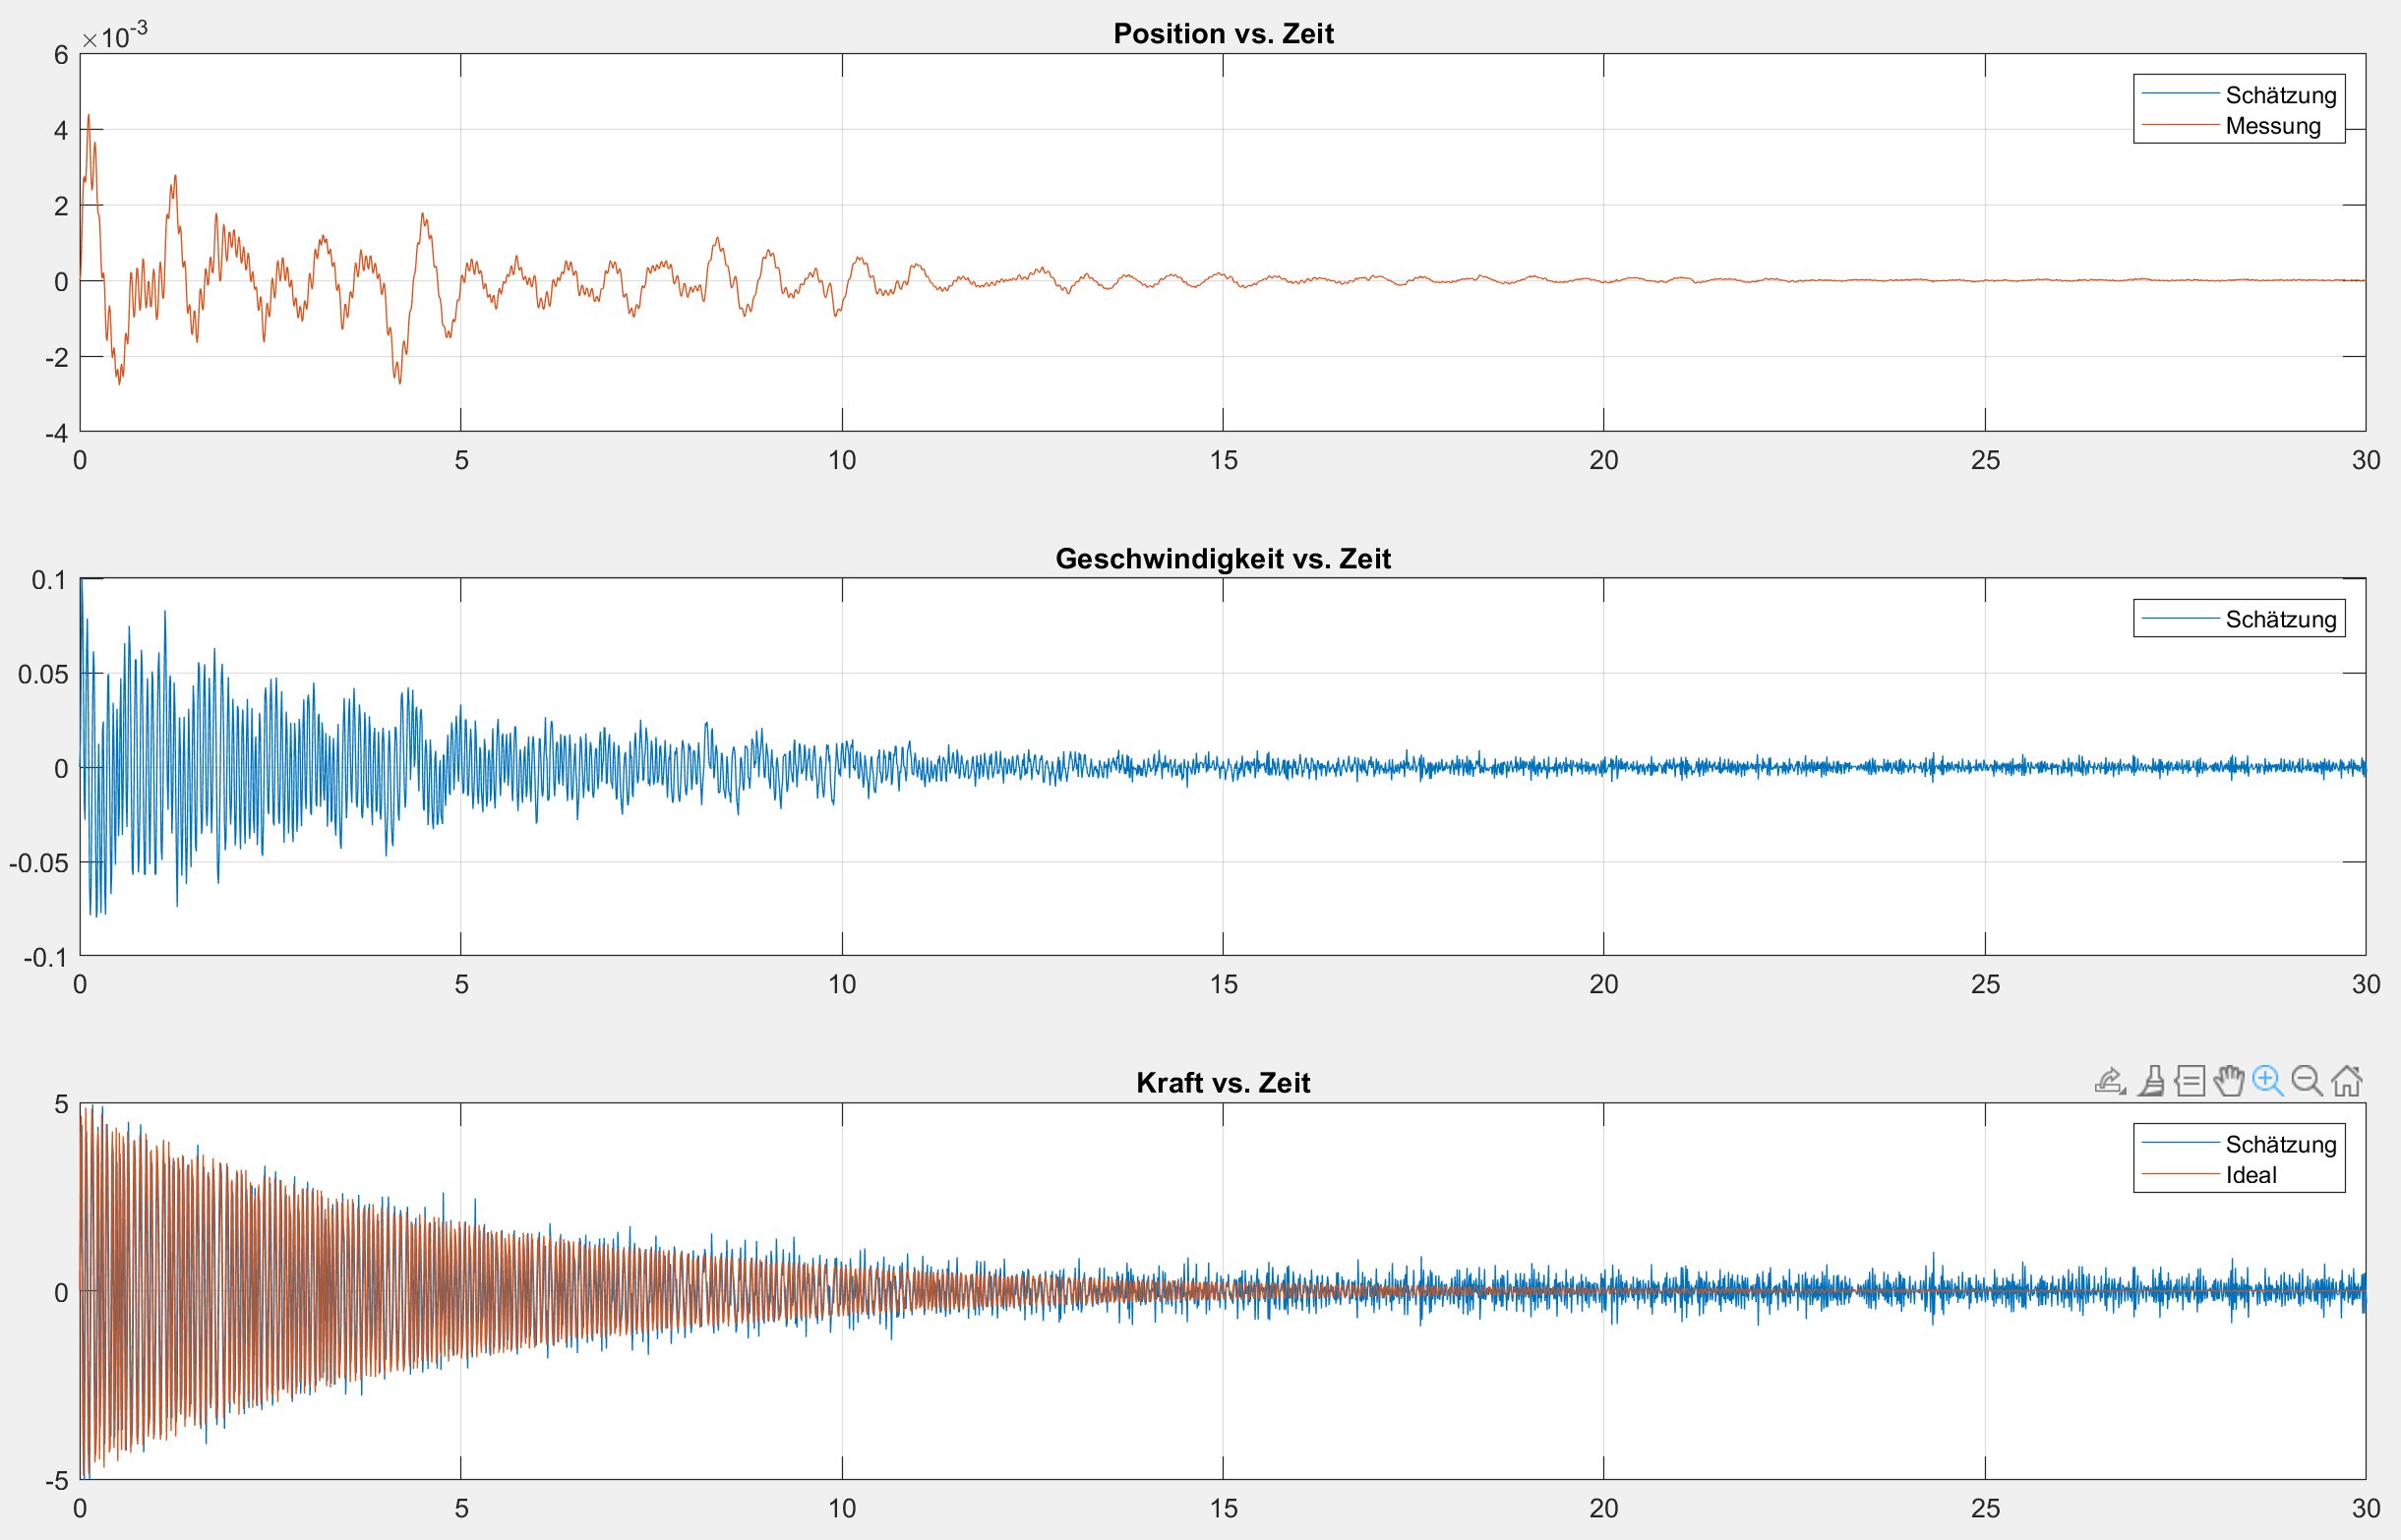
\includegraphics[width=\linewidth,keepaspectratio]{papers/erdbeben/Standard_alles.PNG}
		\caption{Das Position-Zeit-Diagramm zeigt uns die typische Aufzeichnung eines Seismographen während eines Erdbebens. Um die Geschwindigkeit zu erhalten müssen wir die Positionsveränderung einmal ableiten. Ein weiteres Ableiten erzeugt uns die Beschleunigung resp. die Kraft.}
    \label{erdbeben:fig:standard-alles}
	\end{center}
\end{figure}

\begin{figure}
	\begin{center}
		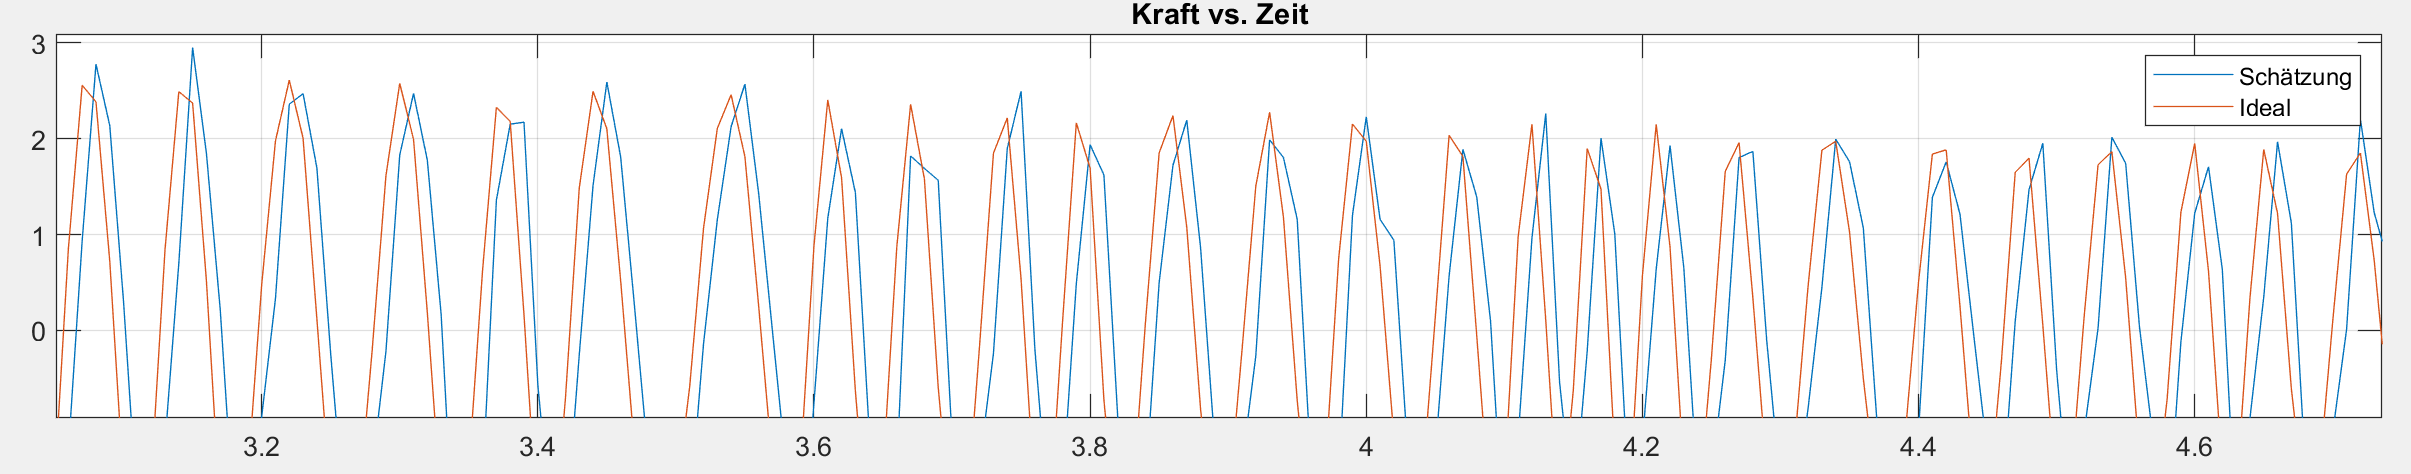
\includegraphics[width=\linewidth,keepaspectratio]{papers/erdbeben/Erdbeben_Standardfall_Zoom.PNG}
		\caption{Erst das Vergrössern an die Datenpunkte zeigt uns auf, wie gut die Schätzung des Kalman-Filters funktioniert.}
    \label{erdbeben:fig:standard-zoom}
	\end{center}
\end{figure}

\subsection{Veränderung der Systemparameter}
Was wir nun austesten möchten, sind die Auswirkungen wenn z.B. der Seismograph andere Systemparameter aufweist.
Wir nehmen an, dass sich im Vergleich zum Standardfall die Masse erhöht, die Federkonstante schwächer und die Bodendämpfung doppelt so stark wirkt.
Somit gilt neu
\[
m = 0.05
\qquad \qquad
D = 0.5
\qquad \text{und} \qquad
k = 0.02.
\]

Da wir mit dieser Anpassung die Trägheit des Seismogrammes erhöht haben, erwarten wir sicher eine langsamere Bewegung der Masse, das heisst die Frequenz wird sich reduzieren.

Betrachten wir die Abbildung~\ref{erdbeben:fig:systemparameter-geaendert} können wir diese Erwartung bestätigen.
Nebst dem bemerken wir eine grössere Auslenkung der Position, die wir auf die höhere Energie der Masse und geringeren Rücklenkkraft der Feder begründen können.

\begin{figure}
	\begin{center}
		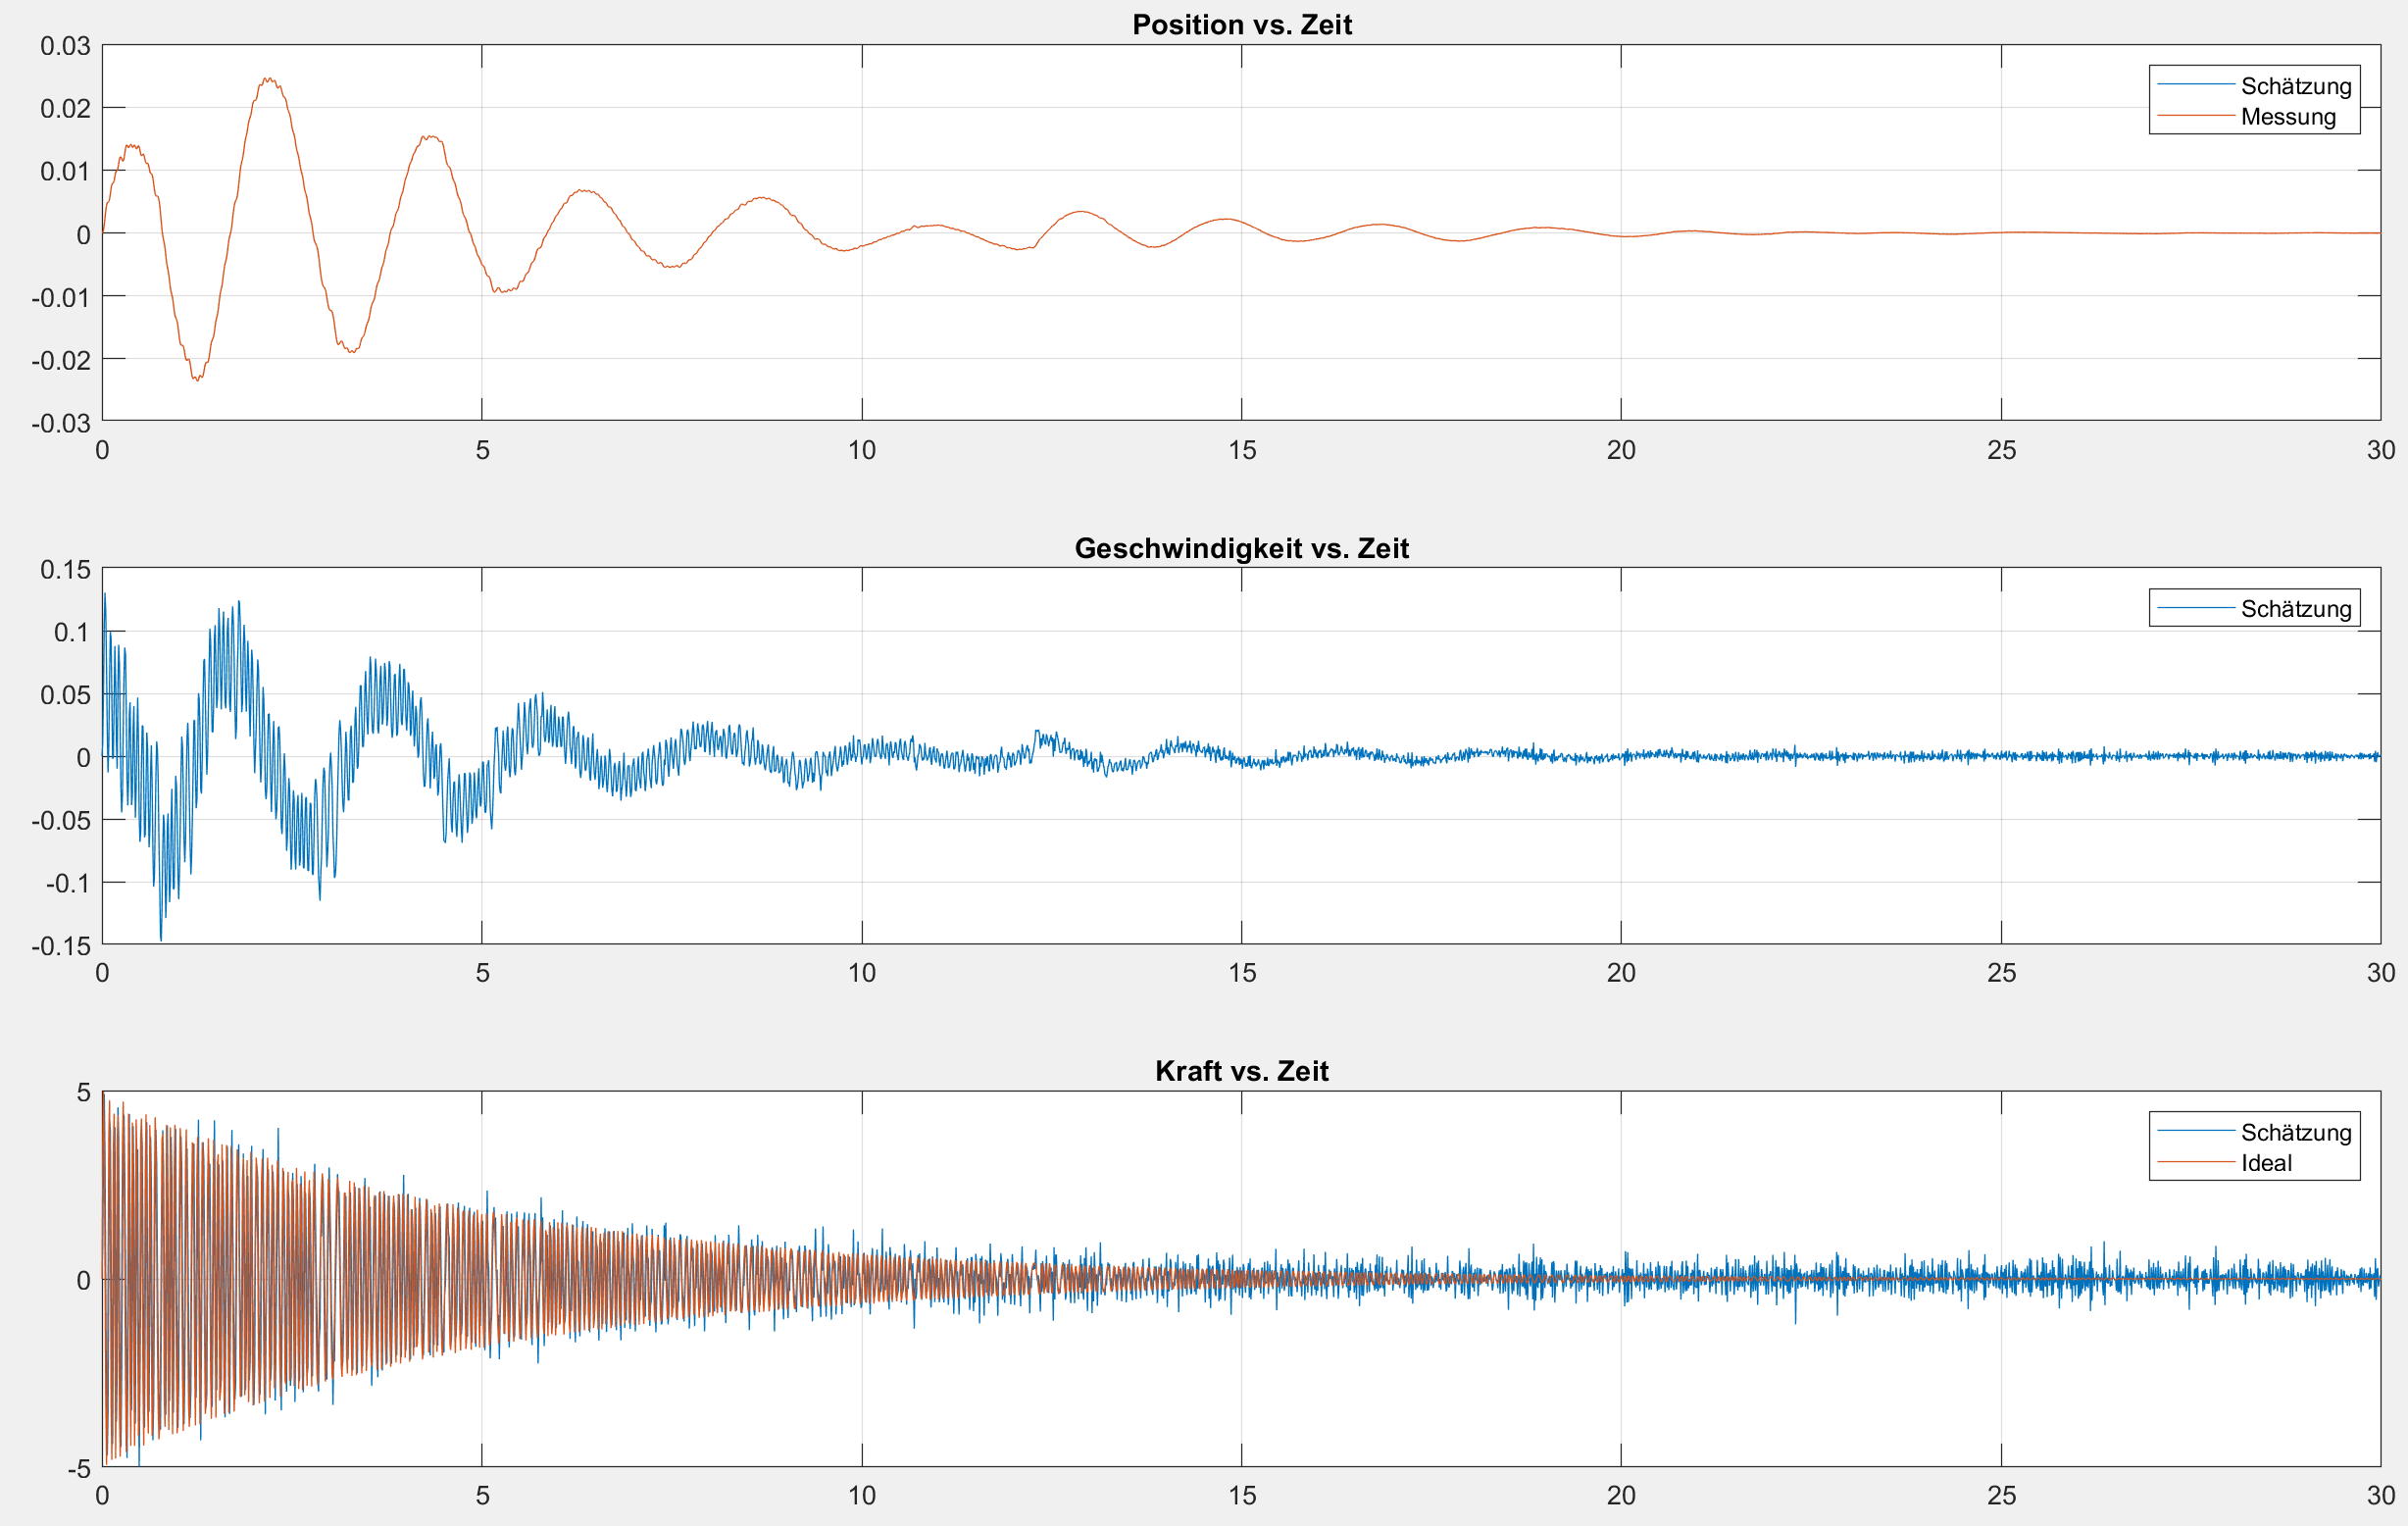
\includegraphics[width=\linewidth,keepaspectratio]{papers/erdbeben/Systemparameter_geaendert_2.PNG}
		\caption{Im Geschwindigkeits-Diagramm erkennen wir in den ersten $6-7$ Sekunden, wie die Erdbebenschwingung die Masse beeinflusst. Gleichzeitig und vorallem im gesamten Zeitverlauf, pendelt sich die Masse in die Eigenschwingung ein.}
    \label{erdbeben:fig:systemparameter-geaendert}
	\end{center}
\end{figure}


\subsection{Verstärkung des Prozessrauschens}
Falls wir unseren Seismographen in der Nähe einer grösseren Stadt aufstellen, so müssen wir aufgrund der Vibrationen mit einem stärkeren Prozessrauschen rechnen.
Dieses Rauschen beeinflusst die Position und Geschwindigkeit in der Zustands-Matrix $Q$.
Aus diesem Grund erhöhen wir die Standardabweichungen in der Matrix $Q$ um den Faktor $1'000$.
Die Auswertung in Abbildung~\ref{erdbeben:fig:prozessrauschen-geaendert} zeigt auf, dass die Kalman-Schätzung der Kraft nur gering an den Messwerten anpasst.

\begin{figure}
	\begin{center}
		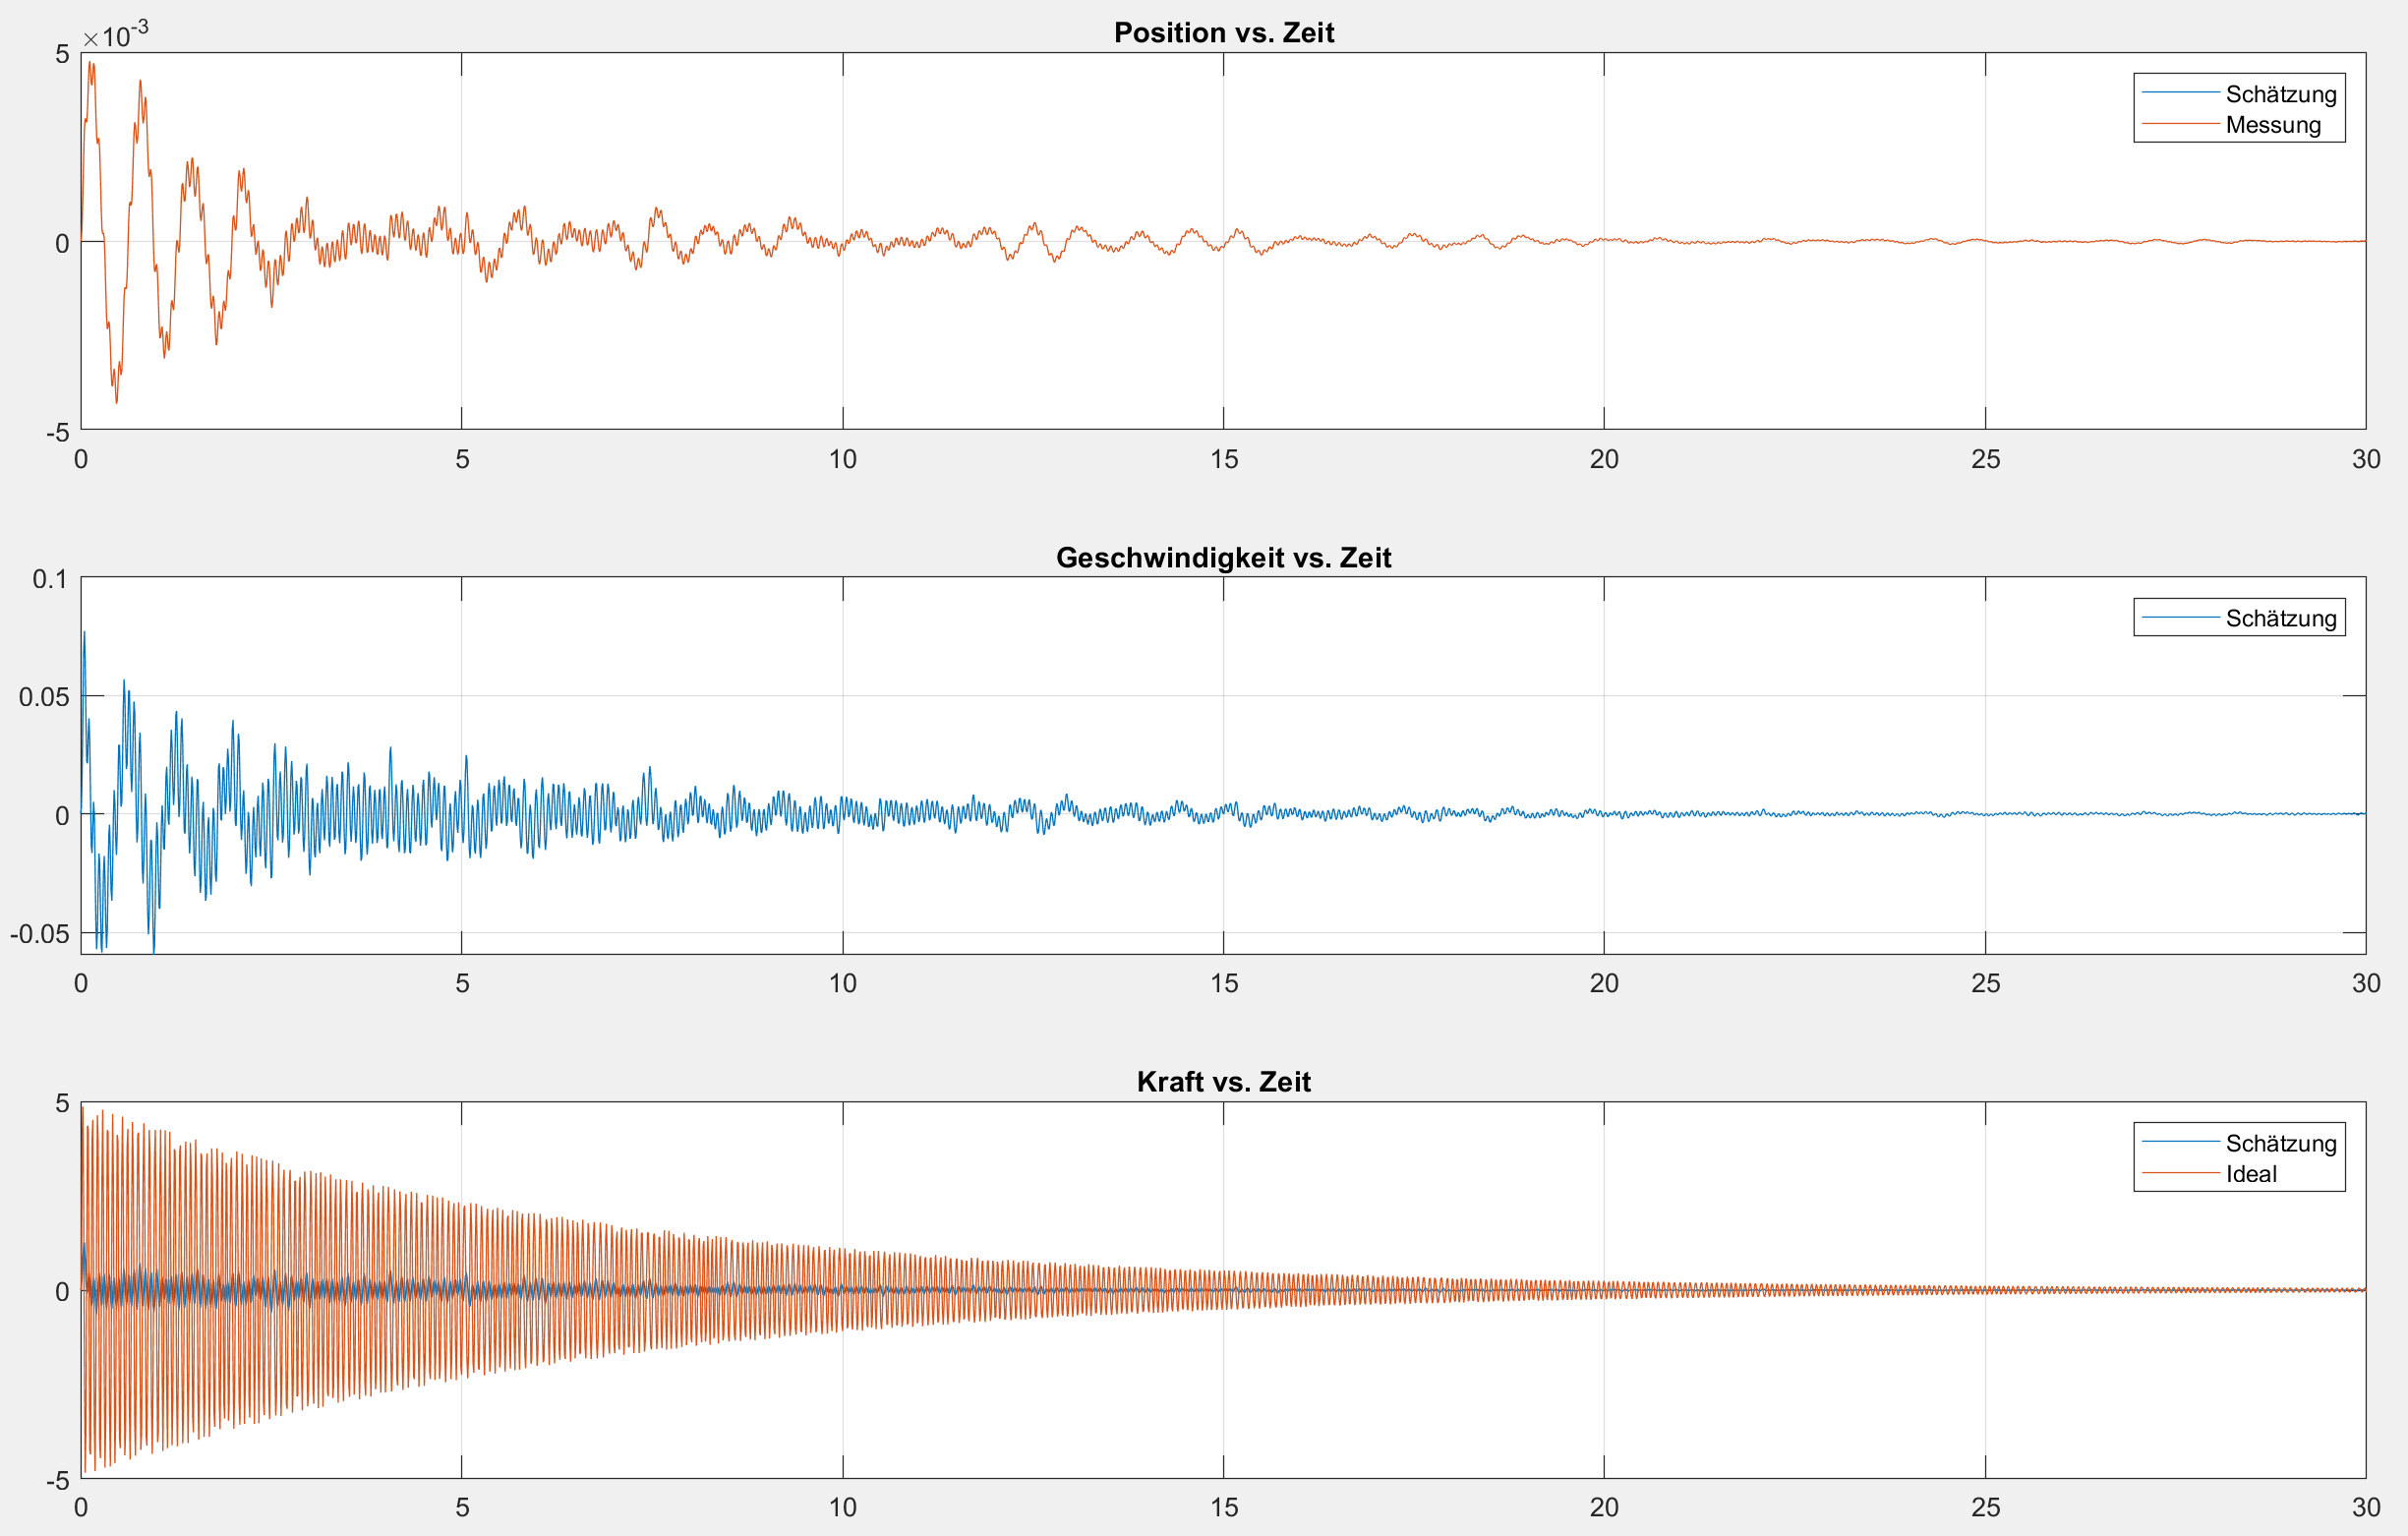
\includegraphics[width=\linewidth,keepaspectratio]{papers/erdbeben/Prozessrauschen_geaendert.PNG}
		\caption{}
    \label{erdbeben:fig:prozessrauschen-geaendert}
	\end{center}
\end{figure}

\subsection{Verstärkung des Messrauschens}
Als letztes verstärken wir das Messrauschen um den Faktor 100 und belassen wieder den Rest wie im Standardfall.
Diese Anpassung bewirkt bei der Position und Geschwindigkeit grosse Abweichungen zwischen der Messgrösse und des Schätzwertes.
Im ganzen ist der Output sehr ungenau und somit nicht mehr brauchbar.

\begin{figure}
	\begin{center}
		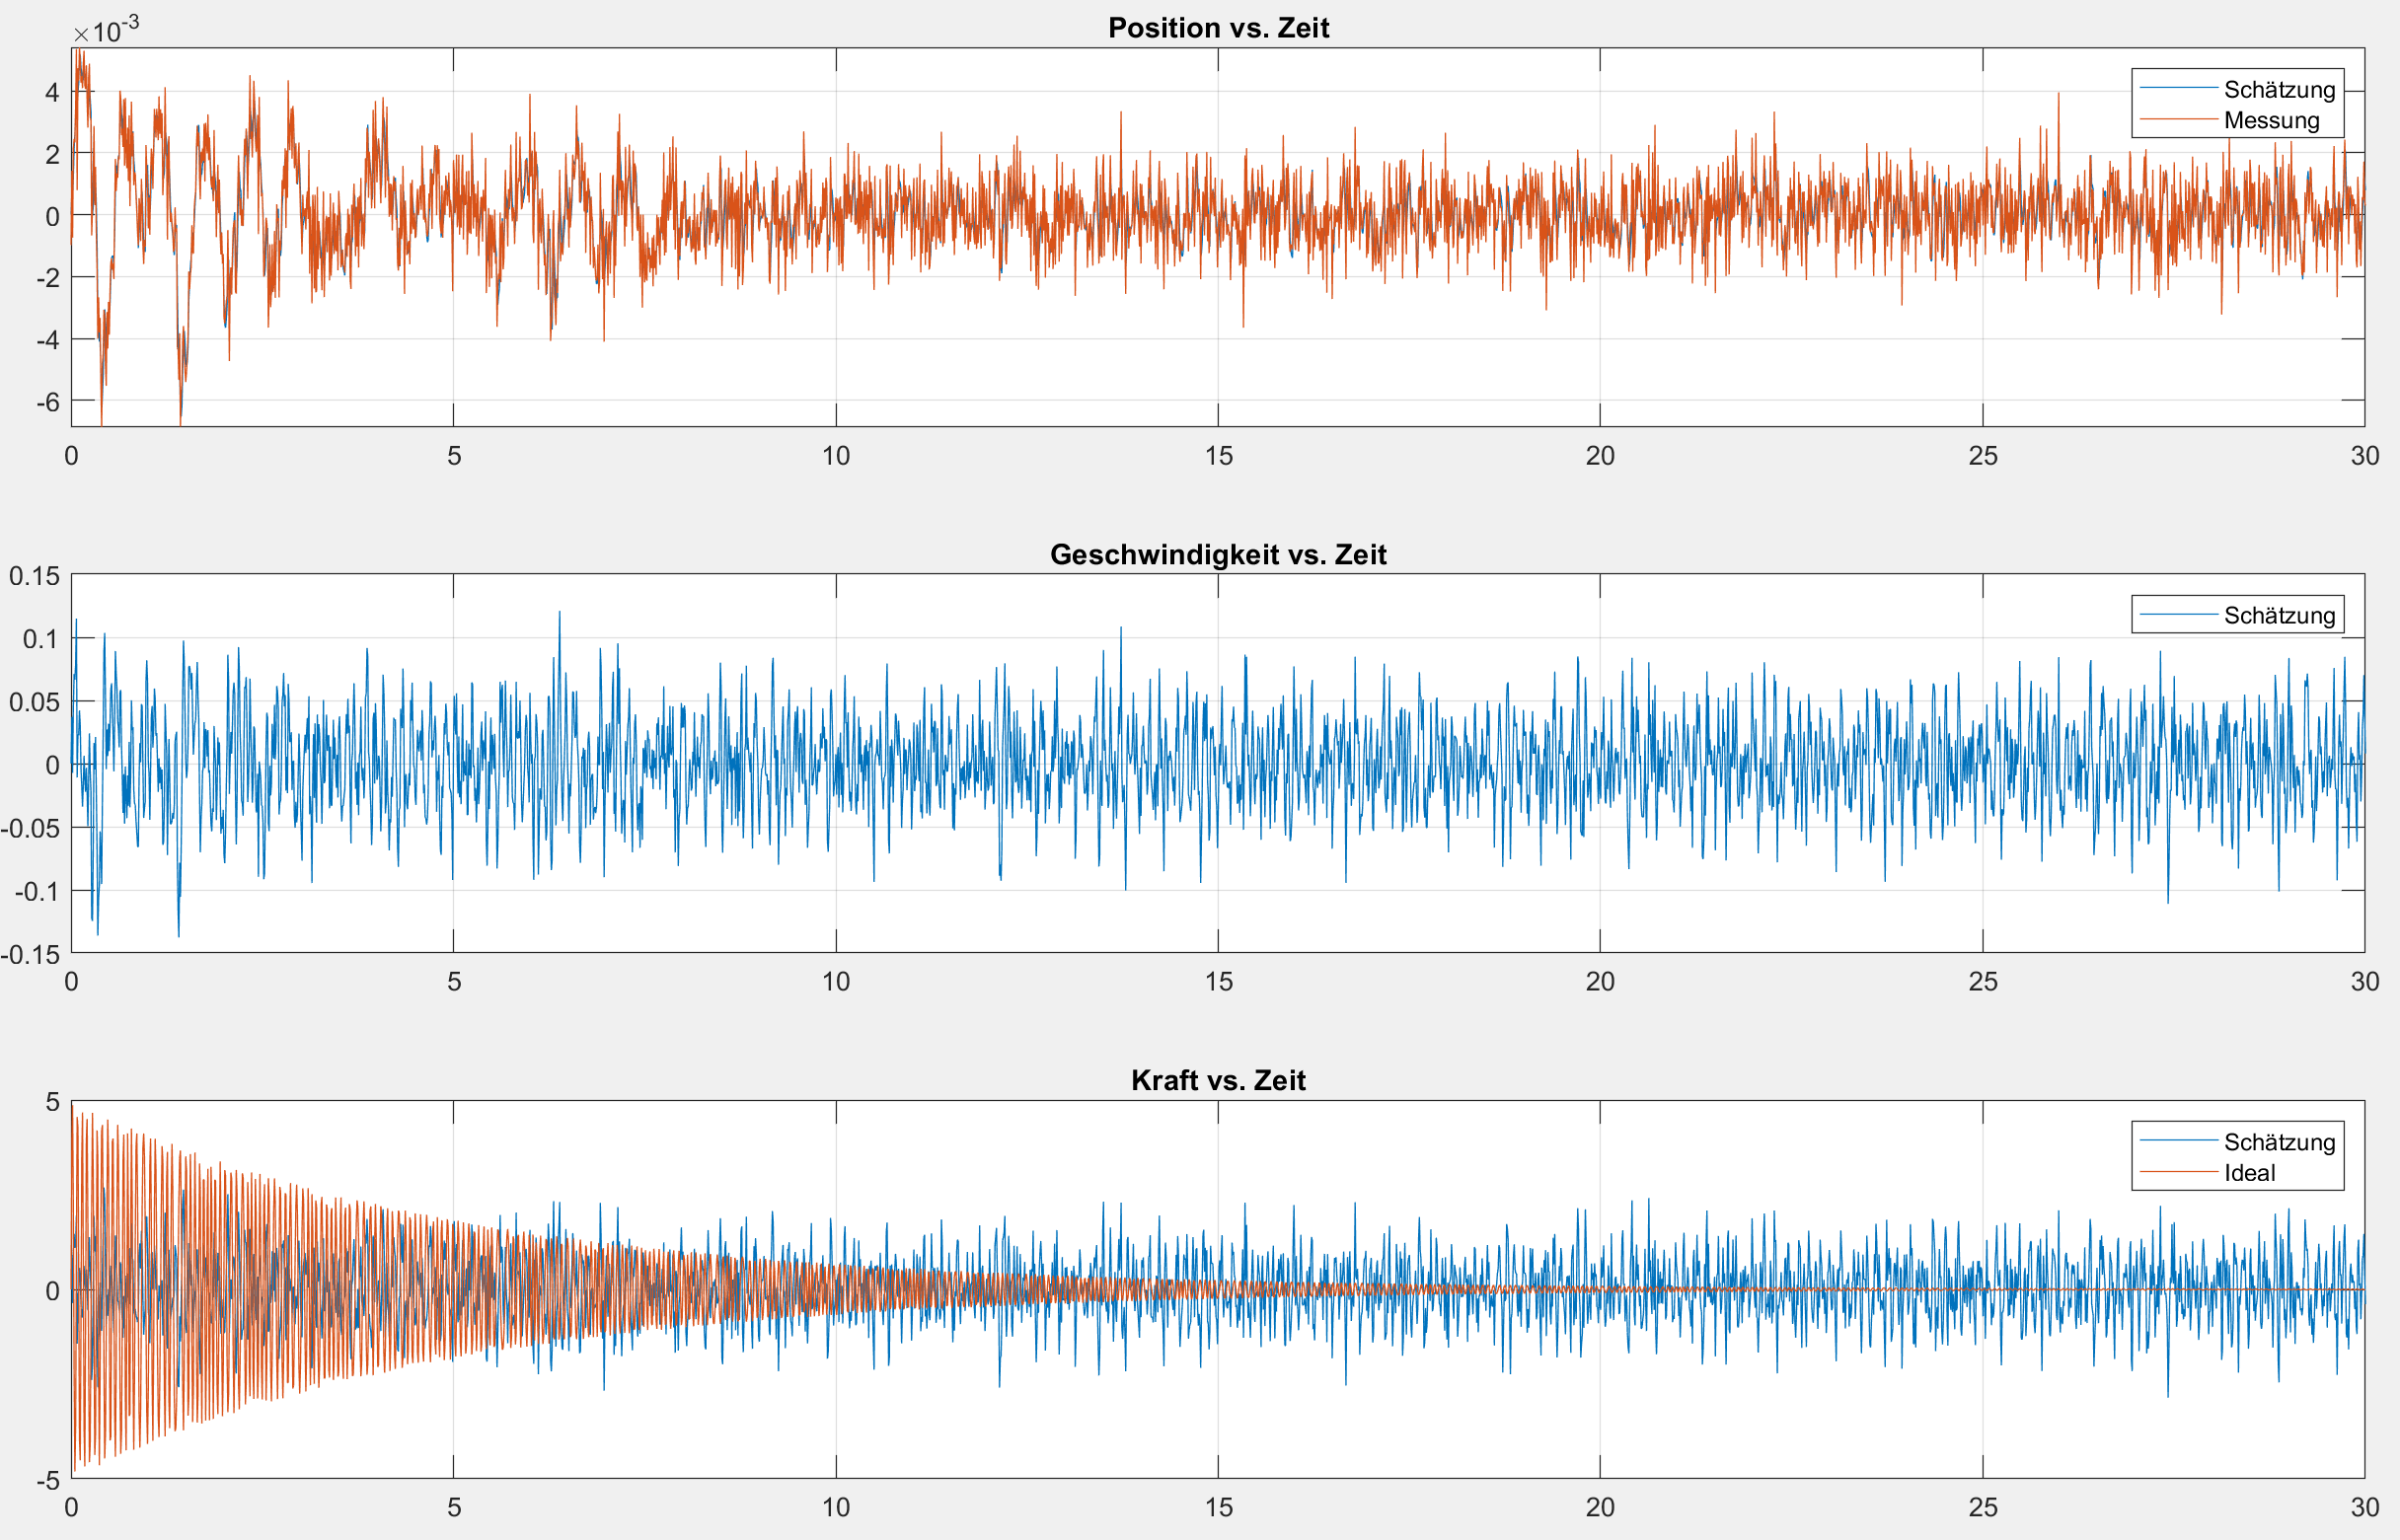
\includegraphics[width=\linewidth,keepaspectratio]{papers/erdbeben/Messrauschen_geaendert.PNG}
		\caption{Das verstärkte Messrauschen dominiert über der Erdbebenschwingung. Die Aufzeichnung wird unbrauchbar und die Schätzung zu ungenau.}
	\end{center}
\end{figure}

